\documentclass[aps,pre,superscriptaddress,amsmath,amssymb,amsfonts,twocolumn,showpacs,notitlepage]{revtex4-1}

% language packages
\usepackage[utf8]{inputenc}
\usepackage[english]{babel}

% math packages
\usepackage{amsmath}
\usepackage{amssymb}
\usepackage{amsfonts}
\usepackage{amstext}
\usepackage{amsthm}
\usepackage{mathtools}

% physics packages
\usepackage{physics}

% bibliography packages
\usepackage{natbib}

% TODO notes
% 
\usepackage{xargs} % Use more than one optional parameter in a new commands
\usepackage[colorinlistoftodos,prependcaption,textsize=tiny]{todonotes}
\newcommandx{\unsure}[2][1=]{\todo[linecolor=red,backgroundcolor=red!25,bordercolor=red,#1]{#2}}
\newcommandx{\change}[2][1=]{\todo[linecolor=blue,backgroundcolor=blue!25,bordercolor=blue,#1]{#2}}
\newcommandx{\info}[2][1=]{\todo[linecolor=OliveGreen,backgroundcolor=OliveGreen!25,bordercolor=OliveGreen,#1]{#2}}
\newcommandx{\improvement}[2][1=]{\todo[linecolor=Plum,backgroundcolor=Plum!25,bordercolor=Plum,#1]{#2}}
\newcommandx{\thiswillnotshow}[2][1=]{\todo[disable,#1]{#2}}
%

% others
\usepackage{graphicx}
\usepackage{bm}
\usepackage{color}
\usepackage[pdftex,dvipsnames]{xcolor}  % Coloured text etc.
\usepackage[colorlinks=true,allcolors=blue]{hyperref}

\begin{document}
	
	\title{Harmonic Oscillator Dynamics using Neural Networks and Stochastic Reconfiguration}
	\date{\today}
	
	\author{Alejandro Romero-Ros}
	\affiliation{Departament de Física Quàntica i Astrofísica (FQA), Universitat de Barcelona (UB),  c. Martí i Franqués, 1, 08028 Barcelona, Spain}
	\affiliation{Institut de Ciències del Cosmos (ICCUB), Universitat de Barcelona (UB), c. Martí i Franqués, 1, 08028 Barcelona, Spain}
	
	\begin{abstract}
		In this document we solve the one-dimensional quantum harmonic oscillator employing two different neural networks, or neural quantum states, as the wavefunction ansätze.
		The first network consists of a single neuron, or perceptron, with a Gaussian activation function.
		The second one, is a common multilayer perceptron.
		In both cases, we use the stochastic reconfiguration method to obtain the ground state and perform subsequent dynamics upon a displacement of the trapping potential.
		Further details can be found in Ref.~\cite{GASP}
	\end{abstract}
		
	\maketitle
	
\section{1D Quantum Harmonic Oscillator} \label{sec:HO}

	The quantum harmonic oscillator (HO) is a well-known textbook example with analytic solution.
	In one dimension (1D), the single-particle Hamiltonian of this system reads
	%
	\begin{equation} \label{eq:hamiltonian}
		\hat{\mathcal{H}} = -\frac{\hbar}{2m}\partial_{x}^2 + \frac{1}{2}m\omega^2\hat{x}^2 \,.
	\end{equation}
	%
	Here, $m$ is the mass of the particle and $\omega$ is the characteristic frequency.
	If we rewrite the above expression in HO units, where energy, length and time are expressed in terms of $\varepsilon_0 =\hbar\omega$, $a_0=\sqrt{\hbar/m\omega}$ and $\tau = \omega^{-1}$, respectively, we obtain the dimensionless Hamiltonian
	%
	\begin{equation} \label{eq:hamiltonian_dimless}
		\hat{\mathcal{H}} = -\frac{1}{2}\partial_{\tilde{x}}^2 + \frac{1}{2}\hat{\tilde{x}}^2 \,.
	\end{equation}
	% 
	with $x'=x/a_0$.
	Note that below we drop the tilde \~{}´ for simplicity.
	The general solution  of Eq.~\eqref{eq:hamiltonian_dimless} (up to a phase) is
	%
	\begin{equation} \label{eq:psi}
		\ket{\psi} = \qty(\frac{1}{\pi})^{\frac{1}{4}}e^{-\frac{1}{2}(x-\ev{x})^2}e^{ix\ev{p}}e^{-\frac{i}{2}\ev{x}\ev{p}} \,.
	\end{equation}
	%
	$\ket{\psi}=\ket{\psi(t)}$ is the wavefunction describing the oscillations of a Gaussian wavepacket, and 
	%
	\begin{align}
		\ev{x}=\ev{x(t)} &= x_0\cos(t) + p_0\sin(t) \,, \label{eq:x(t)}
		\\
		\ev{p}=\ev{p(t)} &= p_0\cos(t) - x_0\sin(t) \,, \label{eq:p(t)}
	\end{align}
	%
	are the position and momentum expectation values, respectively.
	Moreover, it is possible to characterize Eq.~\eqref{eq:psi} employing a single complex-valued parameter
	%
	\begin{align} \label{eq:z(t)}
		z(t) &= \ev{x(t)} + i\ev{p(t)} = z_0e^{-it} \,,
	\end{align}
	%
	with $z_0=x_0+ip_0$.

\section{Stochastic Reconfiguration} \label{sec:SR}

	Assume an ansatz wavefunction $\ket{\psi_{\vec{\theta}}}$ parametrized by a set of $n$ parameters $\vec{\theta} = \{\theta_1,\dots,\theta_n\}$.
	
	The time-evolution of $\ket{\psi_{\vec{\theta}}}$ can be described by the unitary operator $\hat{U}(t)$, so that
	%
	\begin{equation}
		\ket{\psi_{\vec{\theta}}(t)} = \hat{U}(t)\ket{\psi_{\vec{\theta}}} \qq{with} \hat{U}(t)=\exp(-\frac{it}{\hbar}\hat{\mathcal{H}}) \,.
	\end{equation}
	%
	Here, $\hat{\mathcal{H}}$ is the HO Hamiltonian~\eqref{eq:hamiltonian_dimless}.
	
	Additionally, one could also solve the time-evolution of $\ket{\psi_{\vec{\theta}}}$ by changing instead $\vec{\theta}$, so that
	%
	\begin{equation}
		\ket{\psi_{\vec{\theta}(t)}} = \ket{\psi_{\vec{\theta} + \delta t\vec{\theta}}} \,.
	\end{equation}
	
	It can be shown that minimizing the Fubini-Study metric,
	%
	\begin{equation} \label{eq:fubini_metric}
		d(A,B) = \cos^{-1}\sqrt{\frac{\braket{A}{B}\braket{B}{A}}{\braket{A}{A}\braket{B}{B}}} \,,
	\end{equation}
	%
	between the two states $\ket{A}=\ket{\psi_{\vec{\theta}}(t)}$ and $\ket{B}=\ket{\psi_{\vec{\theta} + \delta t\vec{\theta}}}$, yields the evolution equation for the parameters $\vec{\theta}$~\cite{Sinibaldi2023},
	%
	\begin{equation} \label{eq:evolution}
		\bm{S}\dot{\vec{\theta}} = -i\vec{F} \,.
	\end{equation}
	%
	In the expression above, $\bm{S}$ is the quantum geometric tensor (QGT), whose elements read
	%
	\begin{equation}
		S_{jk} = \frac{\braket{\partial_{\theta_j}{\psi_{\vec{\theta}}}}{\partial_{\theta_k}{\psi_{\vec{\theta}}}}}{\braket{\psi_{\vec{\theta}}}} - \frac{\braket{\partial_{\theta_j}\psi_{\vec{\theta}}}{\psi_{\vec{\theta}}}\braket{\psi_{\vec{\theta}}}{\partial_{\theta_k}\psi_{\vec{\theta}}}}{\braket{\psi_{\vec{\theta}}}^2} \,,
	\end{equation}
	%
	and the elements of $\vec{F}$ are the variational forces,
	%
	\begin{equation}
		F_j = \frac{\bra{\partial_{\theta_j}\psi_{\vec{\theta}}}\mathcal{H}\ket{\psi_{\vec{\theta}}}}{\braket{\psi_{\vec{\theta}}}} - \frac{\braket{\partial_{\theta_j}\psi_{\vec{\theta}}}{\psi_{\vec{\theta}}}\bra{\psi_{\vec{\theta}}}\mathcal{H}\ket{\psi_{\vec{\theta}}}}{\braket{\psi_{\vec{\theta}}}^2} \,.
	\end{equation}
	%
	To solve Eq.~\eqref{eq:evolution} one can employ a numerical integrator.
	Additionally, we can also perform imaginary time propagation employing instead the equation $\bm{S}\dot{\vec{\theta}} = -\vec{F}$.

	It is important to recall that $\bm{S}$ is generally found to be a non-invertible matrix, with $\det(\bm{S})=0$, and some methods, such as the Moore-Penrose psudo-inverse, are necessary to compute Eq.~\eqref{eq:evolution}.
	Nevertheless, it is also recommended to regularize $\bm{S}\to\mathcal{R}[\bm{S},\epsilon]$, with $\epsilon\to0$. 

\section{The Neural Network} \label{sec:NN}

	The simplest building block of a neural network (NN) is a perceptron, an artificial neuron-like device that takes input signals, processes them, and signals out an output.
	%
	Typically, a basic NN consists of three main layers, i.e., input, hidden, and output, each conformed by an arbitrary number of perceptrons.
	Moreover, these layers are fully connected with each other neighboring layer, i.e., each perceptron has as many inputs as perceptrons has the previous layer.
	
	One key point of a NN is how the perceptron processes the input data.
	The standard protocol is described by the following expression:
	%
	\begin{equation} \label{eq:perceptron}
		\beta(\vec{\alpha}) = \sigma\qty(\sum_{j=1}^n w_j\alpha_j + b_j) \,,
	\end{equation}
	%
	where $\vec{\alpha}={\alpha_1,\dots,\alpha_n}$ is a set of inputs, $\beta$ is the output, and $\sigma()$ is the so-called activation function.
	Note that the inputs, $\alpha_j$, are modified by weights, $w_j$, and biases, $b_j$, before being evaluated by the activation function.
	These sets of weights and biases are the trainable parameters of the NN.
	
	\todo{explain why NNs are universal function approximators.}
	\todo{explain how the output of the NN is $\psi(\vec{x})$.}
	\todo{explain holomorfism.}
	
\section{Examples} \label{sec:examples}

	In this section we will show different examples increasing the complexity of the network.
	\improvement{NNs figure needed}
	%
	The system under study is the 1D HO described in Sec.~\ref{sec:HO}.
	%
	Moreover, and unless stated otherwise, we will use a finite box with $x_j\in[-8, 8]$ and $n=100$ equidistant grid points, $\vec{x}=$, a 4th order Runge-Kutta method (RK4) to solve Eq.~\eqref{eq:evolution}, and $\mathcal{R}[\bm{S},\epsilon]=\bm{S}+\epsilon$, with $\epsilon=(1+i)\times10^{-5}$.
	
\subsection{Gaussian-activation single-perceptron (GASP) NN} \label{sec:single_NN}

	As we have seen in Sec.~\ref{sec:HO}, it is possible to describe the evolution of a particle in a HO employing a single complex-valued parameter, $z(t)$.
	%
	Therefore, our first NN will consist of a single perceptron (one input and one output) with Eq.~\eqref{eq:psi} as a Gaussian activation function, i.e.,
	%
	\begin{equation} \label{eq:activation_gaussian}
		\sigma(x_j)=  \qty(\frac{1}{\pi})^{\frac{1}{4}}e^{-\frac{1}{2}(x_j-\ev{x})^2}e^{ix_j\ev{p}}e^{-\frac{i}{2}\ev{x}\ev{p}} \,,
	\end{equation}
	%
	with $\ev{x} = \Re(z)$ and $\ev{p}=\Im(z)$.
	
	Since the form of $z(t)$~\eqref{eq:z(t)} is well-known, our objective, as a proof of principle, is to characterize its temporal evolution employing stochastic reconfiguration and compare the analytic solution with the numerical method.
	%
	Explicit expressions for $\bm{S}$ and $\vec{F}$ are provided in the Appendix~\ref{app:help}.
	
	
	Initially, we prepare the system with the harmonic trapping displaced to $x=1$.
	This can be done by the change of variable $\hat{x}\to\hat{x}-x_0$ in Eq.~\eqref{eq:hamiltonian_dimless}, with $x_0=1$.
	For this particular case, we will not show how to obtain the ground state, as the initialization of the parameters is trivial, i.e., $z(t=0)=1$.
	Then, we quench the trap to $x=0$, and thus let the system evolve according to the original Hamiltonian~\eqref{eq:hamiltonian_dimless}.
	The results are presented in Fig.~\ref{fig:single}.
	
	In Fig.~\ref{fig:single}(a), we show the spatiotemporal evolution of $|\psi(x,t)|^2$, where the oscillations inside the trapping potential are clearly seen.
	Additionally, Figs.~\ref{fig:single}(b) and \ref{fig:single}(c) depict the time evolution of the real and imaginary contribution of $z(t)$, corresponding to Eqs.~\eqref{eq:x(t)} and \eqref{eq:p(t)}, respectively.
	%
	In this particular case, we used a RK4 with step size $dt=0.1$.
	Comparing the obtained results with the analytical expressions, presented in Sec.~\ref{sec:HO}, we found differences of order $\mathcal{O}(10^{-5})$.
	Yet, employing a $dt=0.01$, the differences decrease down to $\mathcal{O}(10^{-12})$.  
	
	%	
	\begin{figure} 
		\centering
		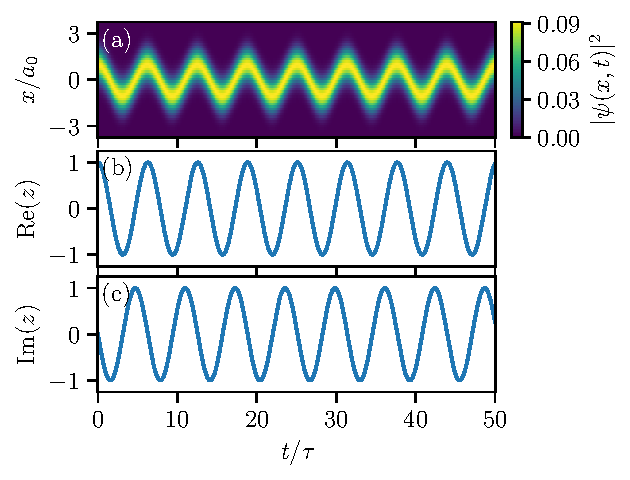
\includegraphics[width=\columnwidth]{single.pdf}
		\caption{
			Time evolution of the Gaussian-activation single-perceptron NN described in Sec.~\ref{sec:single_NN} with a single complex-valued parameter.
			(a) Spatiotemporal evolution of $|\psi(x,t)|^2$.
			(b) and (c) Real and imaginary contributions of $z(t)$, corresponding to Eqs.~\eqref{eq:x(t)} and \eqref{eq:p(t)}, respectively.
			}
		\label{fig:single}
	\end{figure}	
	%
	
	Here, we also considered the case where $\ev{x}$ and $\ev{p}$ are two complex-valued parameters.
	If, once again, we initialize the NN with the trivial solution as described above, i.e., $\ev{x(t=0)}=1$ and $\ev{p(t=0)}=0$, we can directly let the NN evolve according to the Hamiltonian~\eqref{eq:hamiltonian_dimless}.
	The results are presented in Fig.~\ref{fig:double}.
	
	In Fig.~\ref{fig:double}(a) we showcase the spatiotemporal evolution of $| \psi(x,t)|^2$, obtaining the same result as in the previous case [cf. Fig.~\ref{fig:single}(a)].
	%
	Now, in Figs.~\ref{fig:double}(b) and \ref{fig:double}(c) the real and imaginary contribution of each parameter $\vec{\theta}=\qty{\ev{x}, \ev{p}}$ is depicted.
	Analytical expressions for $\ev{x(t)}$ and $\ev{p(t)}$ can be found in the Appendix~\ref{app:help2}.
	
	It is also important to mention that, here, employing a time step $dt=0.1$ in the RK4 yields an error of the order $\mathcal{O}(10^{-2})$.
	Reducing the latter to $dt=0.01$ further decreases the error to an order $\mathcal{O}(10^{-4})$.
	%
	\begin{figure} 
		\centering
		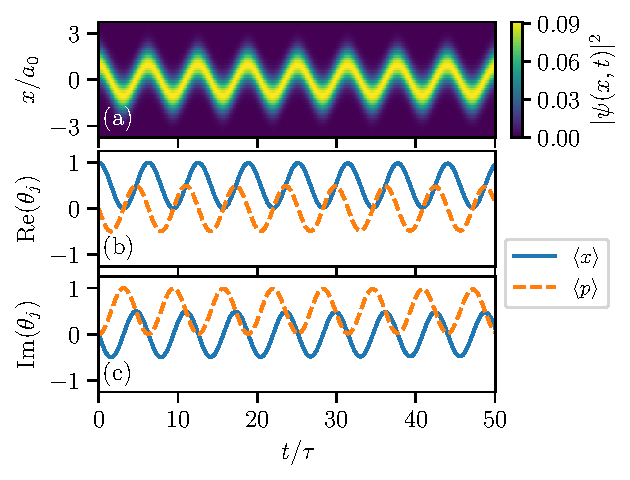
\includegraphics[width=\columnwidth]{double.pdf}
		\caption{
			Time evolution of the Gaussian-activation single-perceptron NN described in Sec.~\ref{sec:single_NN} with two complex-valued parameters.
			(a) Spatiotemporal evolution of $|\psi(x,t)|^2$. 
			(b) and (c) Real and imaginary contributions of $\theta_1 = \ev{x}$ and $\theta_2 = \ev{p}$.
		}
		\label{fig:double}
	\end{figure}
	%
	
\subsection{Multilayer perceptron NN} \label{sec:MLP_NN}
	
	The multilayer perceptron, or neural quantum state (NQS), employed in this example has an extra hidden layer.
	Additionally, its weights and biases are initialized using the Xavier initialization~\cite{Glorot2010} with real valued contribution only.
	%
	Contrary to the GASP (see Sec:~\ref{sec:single_NN}), where the form of the wavefunction was known and used as the activation function, the target wavefunction is unknown.
	Hence, here we use a commonly used sigmoid activation function in all neurons, for complex inputs $z$,
	%
	\begin{equation}
		\sigma(z) = \frac{1}{1+e^{-z}} \,.
	\end{equation}
	%
	The latter implies that more than one parameter will be needed to describe the HO.
	
	For instance, the simplest NQS consists of a single hidden neuron, and a total of 4 parameters, $\theta_j$, (accounting for both weights and biases).
	%
	In Fig.~\ref{fig:NQS_1-1-1_imag}, we showcase the imaginary time evolution of such NQS, in an effort to reach the ground state.
	It is important to mention that one has to pay special attention to the integration method, and the regularization and inversion of $\bm{S}$.
	In this case, we achieve convergence of the energy ($\delta E < 10^{-8}$) using $\epsilon=(1+i)\times10^{-3}$ and a RK4 integration step $\delta t=0.01$.
	However, being able to reach the ground state does not assure convergence during real time evolution.
	The lack of parameters becomes more evident when computing the dynamics, shown in Fig.~\ref{fig:NQS_1-1-1_real}.
	Clearly, the oscillations performed by the NQS in Fig.~\ref{fig:NQS_1-1-1_real}(a) do not correspond to the correct ones [cf. Figs~\ref{fig:single}(a) and \ref{fig:double}(a)].
	
	%
	\begin{figure} 
		\centering
		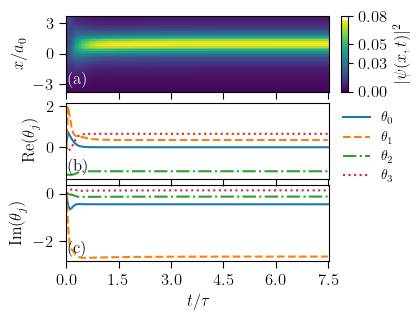
\includegraphics[width=\columnwidth]{NQS_1-1-1_imag.png}
		\caption{
			Imaginary time evolution of the NQS described in Sec.~\ref{sec:MLP_NN} with a single hidden neuron.
			(a) Spatiotemporal evolution of $|\psi(x,t)|^2$. 
			(b) and (c) Real and imaginary contributions of $\vec{\theta}(t)$.
		}
		\label{fig:NQS_1-1-1_imag}
	\end{figure}
	%
	\begin{figure} 
		\centering
		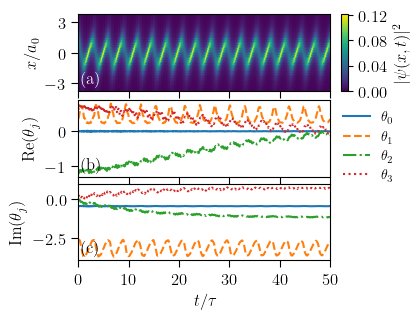
\includegraphics[width=\columnwidth]{NQS_1-1-1_real.png}
		\caption{
			Real time evolution of the NQS described in Sec.~\ref{sec:MLP_NN} with a single hidden neuron.
			(a) Spatiotemporal evolution of $|\psi(x,t)|^2$. 
			(b) and (c) Real and imaginary contributions of $\vec{\theta}(t)$.
			The lack of parameters does not allow the NQS to perform the correct dynamics.
		}
		\label{fig:NQS_1-1-1_real}
	\end{figure}
	%
	
	Of course, one can increase the number of hidden neurons and hidden layers as well.
	In our last example, we employ 2 hidden neurons in the same layer, increasing the number of parameters to 7.
	Fig.~\ref{fig:NQS_1-2-1_imag} depicts the imaginary time evolution of the NQS towards the ground state of the HO.
	Compared to the previous case, shown in Fig.~\ref{fig:NQS_1-1-1_imag}, it takes longer to converge.
	Yet, it is interesting to notice that here we converge to a set of only 3 contributing parameters, and no imaginary contribution.
	
	Unfortunately, the real time evolution dynamics of the NQS, shown in fig.~\ref{fig:NQS_1-2-1_real}, is frustrated by a cumulative error over time due to lack of computational precision, both in the numerical integrator and the regularization and inversion of $\bm{S}$.
	%
	In order to circumvent this problem, smaller integration steps can be performed, and more sophisticated methods can be used around $\bm{S}$, all at its corresponding computational costs.
	
	%
	\begin{figure} 
		\centering
		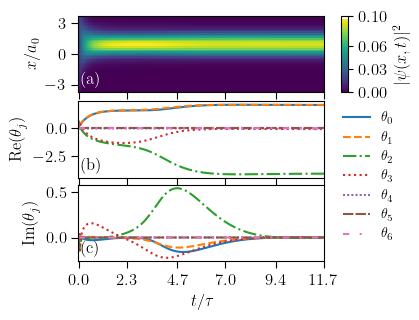
\includegraphics[width=\columnwidth]{NQS_1-2-1_imag_v1.png}
		\caption{
			Imaginary time evolution of the NQS described in Sec.~\ref{sec:MLP_NN} with two hidden neurons.
			(a) Spatiotemporal evolution of $|\psi(x,t)|^2$. 
			(b) and (c) Real and imaginary contributions of $\vec{\theta}(t)$.
		}
		\label{fig:NQS_1-2-1_imag}
	\end{figure}
		%
	\begin{figure} 
		\centering
		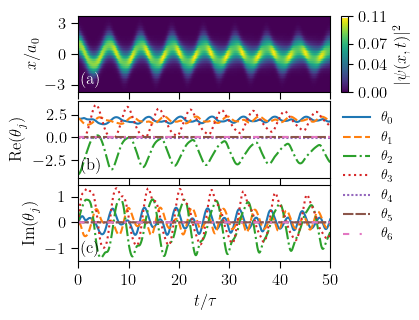
\includegraphics[width=\columnwidth]{NQS_1-2-1_real_v1.png}
		\caption{
			Real time evolution of the NQS described in Sec.~\ref{sec:MLP_NN} with two hidden neurons.
			(a) Spatiotemporal evolution of $|\psi(x,t)|^2$. 
			(b) and (c) Real and imaginary contributions of $\vec{\theta}(t)$.
			An error accumulates over time.
		}
		\label{fig:NQS_1-2-1_real}
	\end{figure}
	%


\clearpage
\appendix
The following calculations can be found in Ref.~\cite{GASP}.
\section{Wirtinger derivatives}
	Given a complex variable $z = x + iy$, with $x,y\in\mathbb{R}$,
	\begin{align}
		\frac{\partial}{\partial z} &= \frac{1}{2}\qty(\frac{\partial}{\partial x} - i\frac{\partial}{\partial y})
		\\
		\frac{\partial}{\partial \bar{z}} &= \frac{1}{2}\qty(\frac{\partial}{\partial x} + i\frac{\partial}{\partial y})
	\end{align}

\section{Helpful calculations - single parameter} \label{app:help}
	With $z = \ev{x} + i\ev{p}$ and  $\ev{x},\ev{p}\in\mathbb{R}$.
	
	Hamiltonian:
	\begin{align}		
		\hat{\mathcal{H}}\ket{\psi} = \frac{1}{2}\left(\ev{p}^2\right.
		&+2 i \ev{p} (x-\ev{x}) \nonumber \\
		&\left.+2 x \ev{x}-\ev{x}^2+1\right)\ket{\psi}		
	\end{align}		
	
	Partial Derivatives:
	\begin{align}
		\ket{\partial_{z}\psi} &= \frac{1}{2}\qty(\ket{\partial_{\ev{x}}\psi} -i\ket{\partial_{\ev{p}}\psi}) \nonumber \\
		&= \frac{1}{4}\qty(4x - 3\ev{x} - i\ev{p})\ket{\psi}
	\end{align}
	
	Expectation values:
	\begin{align}
		\braket{\psi}{\psi} &= 1
		\\		
		\ev{\hat{\mathcal{H}}}{\psi} &= \frac{1}{2}(1+\ev{p}^2+\ev{x}^2) \nonumber \\
		&= \frac{1}{2}\qty(1+|z|^2)
		\\
		\bra{\partial_{z}\psi}\hat{\mathcal{H}}\ket{\psi} &= \frac{1}{8}\qty(\ev{x}+i\ev{p})\qty(5+\ev{x}^2+\ev{p}^2) \nonumber \\
		&= \frac{1}{8}z\qty(5+|z|^2)
		\\
		\braket{\partial_{z}\psi}{\psi} &= \frac{1}{4}(\ev{x} + i\ev{p}) \nonumber \\
		&= \frac{1}{4}z
		\\
		\braket{\partial_{z}\psi}{\partial_{z}\psi} &= \frac{1}{16}(8+\ev{x}^2+\ev{p}^2)\nonumber \\
		& = \frac{1}{16}\qty(8+|z|^2)
	\end{align}
	
	Variational forces:
	\begin{align}
		F_{z} = \frac{1}{2} (\ev{x} + i\ev{p}) = \frac{1}{2}z
	\end{align}
	
	Quantum Geometric Tensor:
	\begin{align}
		S_{z,z} = \frac{1}{2}
	\end{align}
	
	Equations of motion:
	\begin{align}
		\dot{z} &= -iz
	\end{align}
	
\section{Helpful calculations - two parameters} \label{app:help2}

	With $\ev{x}=x_r+ix_i, \ev{p}=p_r+ip_i$ and $x_r,x_i,p_r,p_i \mathbb{R}$.
	
	Hamiltonian:
	\begin{align}		
		\hat{\mathcal{H}}\ket{\psi} = \frac{1}{2}\left(\ev{p}^2\right.
		&+2 i \ev{p} (x-\ev{x}) \nonumber \\
		&\left.+2 x \ev{x}-\ev{x}^2+1\right)\ket{\psi}		
	\end{align}	
	
	Derivatives:
	\begin{align}
		\ket{\partial_{\ev{x}}\psi} &= \qty(x-\ev{x}-\frac{i}{2}\ev{p})\ket{\psi}
		\\
		\ket{\partial_{\ev{p}}\psi} &= \frac{i}{2}(2x-\ev{x})\ket{\psi}		
	\end{align}
	
	Expectation values:
	\begin{align}
		\braket{\psi}{\psi} &= e^{x_i^2}
		\\		
		\ev{\hat{\mathcal{H}}}{\psi} &= \frac{1}{2}\qty(1+\ev{p}^2+\ev{x}^2)e^{x_i^2} \nonumber \\ &+ \qty(\ev{p}-i\ev{x})x_ie^{x_i^2}
		\\
		\bra{\partial_{\ev{x}}\psi}\hat{\mathcal{H}}\ket{\psi} &= \frac{i}{4}\qty(\ev{p}^3+\ev{p}\qty(3+\ev{x}^2)-2i\ev{x}) \nonumber \\
		&+i\qty(\ev{x}^2+\ev{p}^2+1)x_i
		\\
		\bra{\partial_{\ev{p}}\psi}\hat{\mathcal{H}}\ket{\psi} &= -\frac{i}{4}\qty(\ev{x}^3+\ev{x}\qty(3+\ev{p}^2)+2i\ev{p})
		\\
		\braket{\partial_{\ev{x}}\psi}{\psi} &= \frac{i}{2}\ev{p} + 2ix_i
		\\
		\braket{\partial_{\ev{p}}\psi}{\psi} &= -\frac{i}{2}\ev{x}
		\\
		\braket{\partial_{\ev{x}}\psi}{\partial_{\ev{x}}\psi} &= \frac{1}{4}\qty(2+\ev{p}^2) + \ev{p}x_i
		\\
		\braket{\partial_{\ev{p}}\psi}{\partial_{\ev{p}}\psi} &= \frac{1}{4}\qty(2+\ev{x}^2)
		\\
		\braket{\partial_{\ev{x}}\psi}{\partial_{\ev{p}}\psi} &= \frac{1}{4}(2i-\ev{x}\ev{p}) - \ev{x}x_i	
	\end{align}
	
	Variational forces:
	\begin{align}
		F_{\ev{x}} &= \dots
		\\
		F_{\ev{p}} &= \dots
	\end{align}
	
	Quantum Geometric Tensor:
	\begin{align}
		S &=\mqty(  S_{\ev{x},\ev{x}}  & S_{\ev{x},\ev{p}} \\ 
					S_{\ev{p},\ev{x}}  & S_{\ev{p},\ev{p}})
		=\dots
	\end{align}
	
	Equations of motion:
	\begin{align}
		\dot{\theta}_j(t) &= -i\sum_{j}S_{j,k}^{-1}F_{k}
		\\
		\ev{\dot{x}} &= \frac{i(1+\ev{p}^2)+\ev{p}\ev{x}}{\ev{p}^2 + \ev{x}^2}
		\\
		\ev{\dot{p}} &= -\frac{(1+\ev{x}^2)+i\ev{p}\ev{x}}{\ev{p}^2 + \ev{x}^2}
	\end{align}

\bibliographystyle{apsrev4-1}
\bibliography{MyUB_Library}

\newpage
\listoftodos[Notes]
	
\end{document}
